% ข้อเสนอโครงงาน 01204496 — คอมไพล์ด้วย XeLaTeX
%   xelatex proposal.tex   (รันสองครั้งเพื่อให้ \pageref ถูกต้อง)
\documentclass[a4paper,12pt]{article}

\usepackage{fontspec}
\usepackage{geometry}
\usepackage{amsmath}
\usepackage{booktabs}
\usepackage{array}
\usepackage{tabularx}
\usepackage{xcolor}
\usepackage{titlesec}
\usepackage{enumitem}
\usepackage{fancyhdr}
\usepackage{caption}
\usepackage{tikz}
\usetikzlibrary{positioning,arrows.meta,fit,backgrounds,calc}
\usepackage{graphicx}
\usepackage{indentfirst}  % ย่อหน้าแรกหลังหัวข้อก็ต้องเว้าเข้าด้วย
\usepackage[hidelinks]{hyperref}

% ---------- หน้ากระดาษ ----------
\geometry{a4paper,top=2.4cm,bottom=2.4cm,left=2.5cm,right=2.5cm,footskip=1.1cm}

% ---------- ฟอนต์ไทย ----------
% Sarabun คือฟอนต์มาตรฐานของเอกสารราชการไทย มีทั้งอักษรไทยและละตินในตัวเดียว
\setmainfont{Sarabun}[
  Path           = /home/panguin/.fonts/Sarabun/,
  Extension      = .ttf,
  UprightFont    = *-Regular,
  BoldFont       = *-Bold,
  ItalicFont     = *-Italic,
  BoldItalicFont = *-BoldItalic,
  Ligatures      = TeX,
]
\newfontfamily\thaisemi{Sarabun}[
  Path=/home/panguin/.fonts/Sarabun/, Extension=.ttf, UprightFont=*-SemiBold]
\setmonofont{DejaVu Sans Mono}[Scale=0.85]

% การตัดคำภาษาไทย — ภาษาไทยไม่มีช่องว่างระหว่างคำ ต้องให้ ICU ตัดให้
\XeTeXlinebreaklocale "th"
\XeTeXlinebreakskip = 0pt plus 1.2pt minus 0.2pt
\XeTeXlinebreakpenalty = 0
% ผ่อนเกณฑ์การจัดบรรทัด — ภาษาไทยไม่มี hyphenation จึงต้องให้ TeX ยืดช่องไฟได้มากกว่าปกติ
\tolerance = 3000
\emergencystretch = 3em
\hbadness = 4000

\linespread{1.15}
\setlength{\parindent}{2em}
\setlength{\parskip}{0.35em}

% ---------- สี ----------
\definecolor{rule}{HTML}{2F3E4E}
\definecolor{boxfill}{HTML}{EEF2F6}
\definecolor{boxline}{HTML}{51677D}
\definecolor{srcfill}{HTML}{DDE6EE}
\definecolor{accent}{HTML}{1F4E79}

% ---------- หัวข้อ ----------
\titleformat{\section}{\normalsize\bfseries\color{accent}}{\thesection.}{0.6em}{}
\titlespacing*{\section}{0pt}{1.5em}{0.5em}
\titleformat{\subsection}{\normalsize\bfseries}{\thesubsection}{0.6em}{}
\titlespacing*{\subsection}{0pt}{1.0em}{0.3em}

% ---------- หัว-ท้ายกระดาษ ----------
\setlength{\headheight}{15.8pt}
\pagestyle{fancy}
\fancyhf{}
\renewcommand{\headrulewidth}{0.4pt}
\renewcommand{\headrule}{\hrule height 0.4pt width \headwidth \vspace{2pt}}
\fancyhead[L]{\footnotesize 01204496 ข้อเสนอโครงงาน}
\fancyhead[R]{\footnotesize กวินภพ จันเจือ · 6710503739}
\fancyfoot[C]{\footnotesize\thepage}

% หน้าแรกไม่ใส่หัวกระดาษ เพราะซ้ำกับบล็อกชื่อเรื่อง
\fancypagestyle{firstpage}{%
  \fancyhf{}%
  \renewcommand{\headrulewidth}{0pt}%
  \renewcommand{\headrule}{}%   ต้องล้างด้วย เพราะ \headrule ถูก redefine ไว้ข้างบน
  \fancyfoot[C]{\footnotesize\thepage}%
}

% ---------- รายการ ----------
\setlist[enumerate]{topsep=0.2em,itemsep=0.25em,parsep=0.15em,leftmargin=1.6em}
\setlist[itemize]{topsep=0.2em,itemsep=0.25em,parsep=0.15em,leftmargin=1.4em}

% ---------- ตาราง ----------
\renewcommand{\arraystretch}{1.25}
\newcolumntype{L}[1]{>{\raggedright\arraybackslash}p{#1}}
\captionsetup[figure]{font=small,labelfont=bf,skip=6pt,hypcap=false}
\captionsetup[table]{font=small,labelfont=bf,skip=4pt,position=top}

\begin{document}
\thispagestyle{firstpage}

% ============================================================
%  หัวเรื่อง
% ============================================================
\begin{center}
  {\bfseries 01204496 การประมวลผลสัญญาณดิจิทัลเชิงอัลกอริทึมสำหรับวิศวกรคอมพิวเตอร์}\\[1pt]
  {\small Algorithmic-Oriented Digital Signal Processing for Computer Engineers}\\[8pt]
  \textcolor{rule}{\rule{\textwidth}{1.1pt}}\\[6pt]
  {\Large\bfseries ข้อเสนอโครงงาน (Project Proposal)}\\[4pt]
  \textcolor{rule}{\rule{\textwidth}{0.5pt}}
\end{center}

\vspace{0.3em}

\begin{center}
\begin{tabular}{@{}>{\bfseries}l@{\hspace{1.2em}}L{12.2cm}@{}}
\toprule
ชื่อนิสิต   & กวินภพ จันเจือ \\
รหัสนิสิต   & 6710503739 \\
ชื่อโครงงาน & การวิเคราะห์ความสอดคล้องเชิงเวลา--ความถี่ระหว่างระดับน้ำทะเลอันดามันกับ climate index
              หลายตัว ด้วย Multiple Wavelet Coherence \\
\bottomrule
\end{tabular}
\end{center}

% ============================================================
\section{บทนำ (Introduction)}

\subsection{ที่มาและความสำคัญของปัญหา}

สัญญาณที่สนใจคือ time series ของระดับน้ำทะเลรายเดือน จาก tide gauge ที่สถานี Ko Taphao Noi
จังหวัดภูเก็ต ฝั่งทะเลอันดามัน ซึ่งเป็น discrete-time signal ที่มีคาบหลายชั้นซ้อนกัน ตั้งแต่วงรอบ
ตามฤดูกาล 1 ปี ไปจนถึงความแปรปรวนหลายปีและหลายสิบปี

เนื่องจากองค์ประกอบเชิงความถี่เป็นแบบ non-stationary สัญญาณ El Niño ที่คาบ 2--7 ปี ปรากฏแรง
ในบางทศวรรษแล้วหายไปในบางทศวรรษ
การวิเคราะห์จึงต้องใช้ time--frequency plane และเนื่องจากระดับน้ำทะเลถูกขับด้วย
climate index หลายตัวพร้อมกัน ต้องใช้เครื่องมือที่วัดความสัมพันธ์ของ
predictor variable หลายตัวพร้อมกันที่ทุกจุดบน plane นั้น คือ Multiple Wavelet Coherence (MWC)

\subsection{วัตถุประสงค์หลักของโครงงาน}

\begin{enumerate}
  \item เพื่อทดลองใช้ Wavelet Coherence และ Multiple Wavelet Coherence วิเคราะห์ความสัมพันธ์
        ระหว่างระดับน้ำทะเลอันดามันกับ climate index บนระนาบเวลา--ความถี่
  \item เพื่อทดลองใช้ anti-alias filter และ decimation แปลงสัญญาณรายชั่วโมงเป็นรายเดือน
        แล้วตรวจสอบกับค่าอ้างอิงทางการของ PSMSL
\end{enumerate}
\clearpage
\subsection{ขอบเขตของโครงงาน (Scope)}

ศึกษาทะเลเดียวคือทะเลอันดามัน สถานีเดียวคือ Ko Taphao Noi ซึ่งเป็นสถานีที่การทดสอบเบื้องต้น

\begin{center}
\begin{tabular}{@{}L{7.4cm}L{3.0cm}L{4.0cm}@{}}
\toprule
\textbf{สัญญาณ} & \textbf{Sampling rate} & \textbf{ความยาว} \\
\midrule
ระดับน้ำทะเล PSMSL (Ko Taphao Noi) & รายเดือน   & พ.ศ. 2483--2567 \\
ระดับน้ำทะเล UHSLC (Ko Taphao Noi) & รายชั่วโมง & 306,785 จุด \\
Climate index 8 ตัว                & รายเดือน   & ประมาณ 900 เดือน \\
\bottomrule
\end{tabular}
\end{center}

climate index 8 ตัว = 6 ตัวจากงานต้นทาง (Niño3.4, PDO, NAO, SOI, AMO, TPI) + 2 ตัวประจำภูมิภาค
(DMI ซึ่งเป็นดัชนี IOD และ WNPMI ซึ่งเป็นดัชนี monsoon)

ข้อจำกัดของโครงงานมีสองข้อ

\begin{enumerate}
  \item ข้อมูลมี missing value 6.2\% และปี ค.ศ. 2004 สูญหายทั้งปี (ปีสึนามิ) จึงต้องออกแบบวิธี
        gap filling และพก mask ไปตลอดสายการคำนวณ
  \item ศึกษาสถานีเดียว จึงสรุปผลได้เฉพาะทะเลอันดามันไม่มีทะเลที่ที่ใช้เปรียบเทียบ
\end{enumerate}

% ============================================================
\section{วิธีที่นำเสนอ (Proposed Method)}

\subsection{แผนภาพสายงาน}

\begin{center}
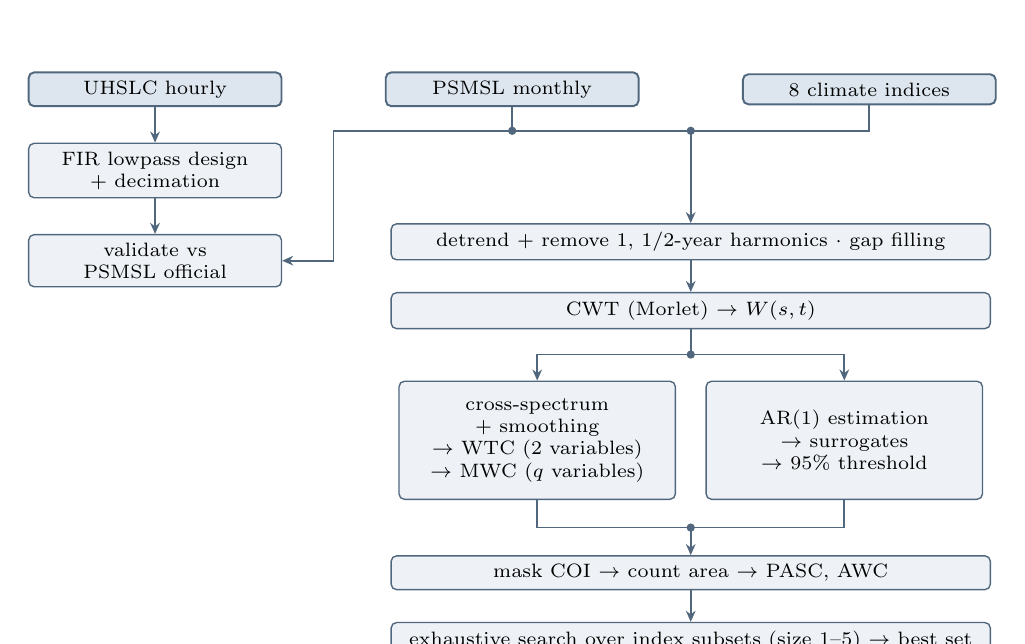
\begin{tikzpicture}[
  node distance = 6mm,
  every node/.style = {font=\scriptsize},
  box/.style   = {rectangle, rounded corners=2pt, draw=boxline, fill=boxfill,
                  line width=0.5pt, align=center, inner sep=3pt, text width=#1},
  src/.style   = {rectangle, rounded corners=2pt, draw=boxline, fill=srcfill,
                  line width=0.7pt, align=center, inner sep=3pt, text width=30mm},
  ar/.style    = {-{Stealth[length=4pt,width=3.5pt]}, draw=boxline, line width=0.6pt},
  ln/.style    = {draw=boxline, line width=0.6pt},                         % เส้นไม่มีหัว ใช้ต่อเข้าจุดแยก/จุดรวม
  dot/.style   = {circle, fill=boxline, inner sep=0pt, minimum size=3pt},  % จุดที่เส้นแยกหรือรวมกัน
]

% --- แถวบน: แหล่งข้อมูล ---
\node[src] (uh)  {UHSLC hourly};
\node[src, right=13mm of uh] (ps) {PSMSL monthly};
\node[src, right=13mm of ps] (ci) {8 climate indices};

% --- สาขาซ้าย: โซ่กรอง ---
\node[box=30mm, below=4.5mm of uh] (fir) {FIR lowpass design\\+ decimation};
\node[box=30mm, below=4.5mm of fir] (val) {validate vs\\PSMSL official};

% --- สายหลัก ---
\coordinate (mid) at ($(ps)!0.5!(ci)$);
\node[box=74mm, below=17mm of mid] (pre)
  {detrend + remove 1, 1/2-year harmonics $\cdot$ gap filling};
\node[box=74mm, below=4mm of pre] (cwt) {CWT (Morlet) $\rightarrow$ $W(s,t)$};

% --- แยกสองสาขา: ซ้าย = สเปกตรัม · ขวา = นัยสำคัญ
%     ตั้งความสูงเท่ากัน เส้นที่ออกจากใต้กล่องจะได้อยู่ระดับเดียวกัน ไม่ซ้อนกัน ---
\node[box=33mm, minimum height=15mm, below=6.5mm of cwt, xshift=-19.5mm] (xs)
  {cross-spectrum + smoothing\\$\rightarrow$ WTC (2 variables)\\$\rightarrow$ MWC ($q$ variables)};
\node[box=33mm, minimum height=15mm, below=6.5mm of cwt, xshift=19.5mm] (ar)
  {AR(1) estimation\\$\rightarrow$ surrogates\\$\rightarrow$ 95\% threshold};

\coordinate (bb) at ($(xs.south)!0.5!(ar.south)$);
\node[box=74mm, anchor=north] (met) at ([yshift=-7mm]bb)
  {mask COI $\rightarrow$ count area $\rightarrow$ PASC, AWC};
\node[box=74mm, below=4mm of met] (srch)
  {exhaustive search over index subsets (size 1--5) $\rightarrow$ best set};

% --- จุดแยก/จุดรวม ---
\coordinate (jp) at ([yshift=-3mm]ps.south);       % PSMSL แยกเป็นสองทาง
\coordinate (jc) at (jp -| pre.north);             % PSMSL กับ climate index รวมกันก่อนเข้าสายหลัก
\coordinate (gx) at ($(uh.east)!0.5!(ps.west)$);   % ช่องว่างระหว่างคอลัมน์ ใช้เดินเส้นไป validate
\coordinate (j1) at ([yshift=-3.2mm]cwt.south);    % CWT แยกสองสาขา
\coordinate (j2) at ([yshift=-3.5mm]bb);           % สองสาขารวมกลับ

% --- เส้นเชื่อม ---
\draw[ar] (uh) -- (fir);
\draw[ar] (fir) -- (val);
\draw[ln] (ps.south) -- (jp);
\draw[ar] (jp) -- (jp -| gx) -- (gx |- val.east) -- (val.east);  % อ้อมตามช่องว่าง ไม่ผ่ากล่อง FIR
\draw[ln] (jp) -- (jc);
\draw[ln] (ci.south) |- (jc);
\draw[ar] (jc) -- (pre.north);
\draw[ar] (pre) -- (cwt);
\draw[ln] (cwt.south) -- (j1);
\draw[ar] (j1) -| (xs.north);
\draw[ar] (j1) -| (ar.north);
\draw[ln] (xs.south) |- (j2);
\draw[ln] (ar.south) |- (j2);
\draw[ar] (j2) -- (met.north);
\draw[ar] (met) -- (srch);
\foreach \p in {jp, jc, j1, j2} \node[dot] at (\p) {};
\end{tikzpicture}
\captionof{figure}{สายงานของโครงงาน ตั้งแต่ข้อมูลดิบจนถึงการค้นหาชุด climate index ที่ดีที่สุด}
\end{center}

\clearpage
\subsection{ทฤษฎีและสมการหลัก}

Cross-wavelet spectrum --- ขยาย cross-spectrum ให้มีความละเอียดเชิงเวลาและความถี่พร้อมกัน

Wavelet Coherence (WTC) --- Grinsted et al.\ (2004) เป็นเหมือน correlation
coefficient ที่ระบุตำแหน่งได้ทั้งในเวลาและความถี่ ตัวอย่างผลลัพธ์จากงานต้นทางแสดงในรูปที่~2

\begin{figure}[tbp]
\centering
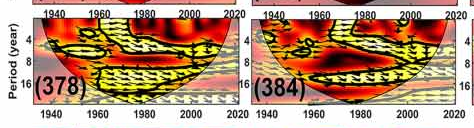
\includegraphics[width=0.74\textwidth]{fig-wtc-example.png}
\caption{ตัวอย่างผลลัพธ์ของ Wavelet Coherence จากงานต้นทาง (ที่มา: Song \& Chen 2022, CC BY 4.0)}
\end{figure}

Multiple Wavelet Coherence (MWC) --- Hu \& Si (2016) ขยาย WTC จาก 2 ตัวแปรเป็น $q$ ตัวแปร
โดยใช้เมทริกซ์ของ auto/cross-spectrum ที่ผ่าน smoothing 

\begin{equation*}
  \rho_m^2(s,t)=\frac{\widetilde{W}^{\,Y,X}\;\left[\widetilde{W}^{\,X,X}\right]^{-1}\;\widetilde{W}^{\,Y,X*}}
  {\widetilde{W}^{\,Y,Y}}
\end{equation*}

Significance test --- ประมาณ AR(1) จากข้อมูลจริงด้วย lag-1 autocorrelation
แล้วสร้าง surrogate ส่งผ่านสายงานเดียวกัน เพื่อหา significance threshold ที่ percentile
ที่ 95 แยกตาม scale

\begin{equation*}
  z_n = a\,z_{n-1} + \varepsilon_n,\qquad \varepsilon_n \sim \mathcal{N}(0,\sigma^2)
\end{equation*}

ตัววัดผล --- นับพื้นที่เฉพาะภายใน Cone of Influence (COI) บนแกน scale แบบ logarithmic

\begin{equation*}
  \mathrm{PASC}=100\times\frac{A_{\mathrm{sig}}}{A_{\mathrm{sig}}+A_{\mathrm{insig}}}
  \qquad\qquad
  \mathrm{AWC}=\overline{\rho^{\,2}}\;\Big|_{\mathrm{significant\ region}}
\end{equation*}
\clearpage
\subsection{function ที่ใช้}

\begin{table}[htbp]
\centering
\caption{การแบ่งงานระหว่างสิ่งที่ใช้จากไลบรารีเดิมกับสิ่งที่สร้างเอง}
\footnotesize
\begin{tabular}{@{}L{4.7cm}L{6.1cm}L{3.5cm}@{}}
\toprule
\textbf{ขั้นตอน} & \textbf{มีให้ใช้แล้วหรือไม่} & \textbf{แผน} \\
\midrule
CWT (Morlet) + scales + COI          & มี --- \texttt{pycwt.cwt}             & ใช้ของงานต้นทาง \\
Smoothing operator                    & มี --- \texttt{pycwt.Morlet().smooth()} & ใช้ของงานต้นทาง \\
Cross-wavelet spectrum                & มี --- \texttt{pycwt.xwt}             & ใช้ของงานต้นทาง \\
Wavelet Coherence (2 ตัวแปร)          & มี --- \texttt{pycwt.wct}             & ใช้เป็นตัวตรวจ ตัวงานได้มาจาก MWC ที่ $q=1$ \\
ประมาณค่า AR(1)                       & มี --- \texttt{pycwt.ar1}             & ใช้ของงานต้นทาง \\
สร้าง AR(1) surrogate                 & มี --- \texttt{pycwt.rednoise}        & ใช้ของงานต้นทาง \\
Significance threshold (2 ตัวแปร)     & มี --- \texttt{pycwt.wct\_significance} (Monte Carlo 300 ชุด) & ใช้ของงานต้นทาง \\
\addlinespace[2pt]
MWC ($q$ ตัวแปร)                      & ไม่มีในไลบรารีไพธอนใดเลย มีแต่โค้ด MATLAB ของ Hu \& Si (2016)
                                        และแพ็กเกจ R ที่ไม่อัปเดตตั้งแต่ปี 2021 & สร้างเอง \\
Significance threshold ของ MWC        & ไม่มี --- \texttt{wct\_significance} รองรับแค่ 2 ตัวแปร & สร้างเอง \\
PASC / AWC                            & ไม่มีในไลบรารีใดเลย                   & สร้างเอง \\
Anti-alias FIR + decimation           & \texttt{scipy.signal} มีบล็อกพื้นฐานให้ & ออกแบบเอง \\
\bottomrule
\end{tabular}
\end{table}

\subsection{เครื่องมือที่ใช้}

\begin{center}
\begin{tabular}{@{}L{4.6cm}L{9.8cm}@{}}
\toprule
\textbf{ประเภท} & \textbf{รายการ} \\
\midrule
ภาษาและสภาพแวดล้อม     & Python 3.12+ จัดการด้วย \texttt{uv} \\
Library ที่ใช้ได้        & \texttt{numpy}, \texttt{scipy}, \texttt{matplotlib}, \texttt{pytest} \\
Library ที่ใช้เป็นฐาน    & \texttt{pycwt} --- รายละเอียดการแบ่งงานอยู่ในหัวข้อ 2.3 \\
ฮาร์ดแวร์               & คอมพิวเตอร์ส่วนตัว \\
แหล่งข้อมูล             & PSMSL, UHSLC, NOAA Physical Sciences Laboratory \\
\bottomrule
\end{tabular}
\end{center}

% ============================================================
\clearpage
\section{ผลลัพธ์ที่คาดหวัง (Expected Outcomes)}

\begin{enumerate}
  \item ภาพ time--frequency plane ของ Wavelet Coherence ระหว่างระดับน้ำทะเลที่ Ko Taphao Noi
        กับ climate index แต่ละตัว
  \item ตาราง PASC และ AWC ของ climate index ทั้ง 8 ตัว 
  \item หาได้ว่า climate index กี่ตัวและชุดใดจึงอธิบายระดับน้ำทะเลอันดามันได้ดีที่สุด
\end{enumerate}

% ============================================================
\section{เกณฑ์การประเมิน (Evaluation Criteria)}

\begin{center}
\footnotesize
\begin{tabular}{@{}L{1.9cm}L{3.5cm}L{8.9cm}@{}}
\toprule
\textbf{ด้าน} & \textbf{เกณฑ์} & \textbf{วิธีวัดและเป้าหมาย} \\
\midrule
ความถูกต้อง & \textbf{MWC}
  & เมื่อกำหนด $q = 1$ ค่า MWC ต้องยุบกลับเป็น WTC ตามนิยาม --- เทียบกับ \texttt{pycwt.wct}
    ต้องต่างไม่เกิน 0.05 ในย่านคาบ 2--7 ปี \\
ความถูกต้อง & \textbf{Filter chain + decimation}
  & นำข้อมูลรายชั่วโมงผ่าน chainเทียบกับค่าเฉลี่ยรายเดือนทางการของ PSMSL
    --- รายงาน RMSE พร้อมอธิบายที่มาของผลต่างที่เหลือ \\
ความถูกต้อง & \textbf{Stopband attenuation}
  & ป้อนสัญญาณทดสอบที่มีความถี่สูงกว่า Nyquist ใหม่ แล้ววัด attenuation
    --- ต้องไม่ปรากฏใน spectrum ของสัญญาณที่ decimate แล้ว \\
ความถูกต้อง & \textbf{การทำซ้ำผลอ้างอิง}
  & ทำซ้ำค่าที่วัดไว้ล่วงหน้าด้วย library คือ $p \approx 0.016$ ที่ Ko Taphao Noi ในย่านคาบ 2--7 ปี \\
\addlinespace[2pt]
คุณภาพผล & \textbf{ตัวชี้วัด}
  & ค่า PASC และ AWC ของแต่ละชุด index $\cdot$ index ที่เพิ่มแล้วทำให้ PASC สูงขึ้น
    อย่างน้อย 5 percentage point จึงถือว่าสำคัญ \\
คุณภาพผล & \textbf{False positive rate}
  & สร้าง synthetic index จาก AR(1) ล้วน ส่งผ่านสายงานเดียวกัน --- ค่า PASC ที่ได้คือ
    \textit{false-positive floor} ที่ผลจริงต้องสูงกว่าจึงมีความหมาย \\
คุณภาพผล & \textbf{Robustness ของข้อสรุป}
  & ทำ sensitivity test โดยเปลี่ยนวิธี gap filling ตัดปีสึนามิออก และตัด index
    ที่จำกัดหน้าต่างเวลาออก \\
คุณภาพผล & \textbf{ความสอดคล้องเชิงกายภาพ}
  & ปีที่พบ significant coherence ต้องตรงกับปีที่เกิด El Niño และ La Niña ที่บันทึกไว้ \\
\bottomrule
\end{tabular}
\end{center}

% ============================================================
\clearpage
\section*{เอกสารอ้างอิง}
\vspace{-0.3em}
{\small
\begin{enumerate}[leftmargin=1.8em,itemsep=0.15em,parsep=0pt]
  \item Song, C. \& Chen, X. (2022). Multivariate analysis of multiscale periodicity in North
        American annual mean sea level based on wavelet coherence and multiple wavelet coherence.
        \textit{Journal of Water and Climate Change}, \textbf{13}(9), 3435--3457.
  \item Grinsted, A., Moore, J. C. \& Jevrejeva, S. (2004). Application of the cross wavelet
        transform and wavelet coherence to geophysical time series.
        \textit{Nonlinear Processes in Geophysics}, \textbf{11}, 561--566.
  \item Hu, W. \& Si, B. C. (2016). Technical note: Multiple wavelet coherence for untangling
        scale-specific and localized multivariate relationships in geosciences.
        \textit{Hydrology and Earth System Sciences}, \textbf{20}, 3183--3191.
  \item Torrence, C. \& Compo, G. P. (1998). A practical guide to wavelet analysis.
        \textit{Bulletin of the American Meteorological Society}, \textbf{79}(1), 61--78.
  \item Torrence, C. \& Webster, P. (1999). Interdecadal changes in the ENSO--monsoon system.
        \textit{Journal of Climate}, \textbf{12}, 2679--2690.
\end{enumerate}
}

\end{document}
